\typeout{IJCAI-09 Instructions for Authors}
\documentclass{article}

\usepackage[letterpaper,margin=0.75in]{geometry}
% \usepackage{amsmath}
% \usepackage{booktabs}
% \usepackage{graphicx}
% \usepackage{listings}
% \usepackage{mathtools}
% \usepackage{fixltx2e}
% \usepackage{hyperref}
% \usepackage{color}
% \usepackage{setspace}
% The file ijcai09.sty is the style file for IJCAI-09 (same as ijcai07.sty).
\usepackage{ijcai09}
% Use the postscript times font!
\usepackage{times}
\usepackage{graphicx}
% \usepackage{url}
% \usepackage{biblatex}
% \bibliography{final_report.bib}

\begin{document}
    \title{News Classifier Group Project}
    \author{Wilson Fearn, Andrew Hale, Victor Lazaro, Spencer Seeger}
    \date{April 10, 2018}
    \maketitle
    \section{Abstract}
    A machine learning approach was applied to the classification of articles found online. 
    Several different machine learning algorithms (Na\"ive Bayes, Random Forest, and 
    Support Vector Machine (SVM)) were applied to a set of 8 categories. 
    After running these models, we found that the better machine learning algorithms were 
    accurate about 95\% of the time. This project can be applied to the real world for 
    companies such as Facebook\textsuperscript{\textregistered} or 
    Google\textsuperscript{\textregistered} when those companies try to suggest articles 
    for a specific user to read.

    \section{Introduction}
    There are many different articles in the world today (either online or printed) with many more 
    continuously being produced. With so many articles being created, it is hard to tell if a reader 
    will appreciate what the article is about. While it is simple enough for a reader to read and 
    discover on their own if they like the article, it would be much easier for the reader to have an 
    already narrowed down selection of articles that they would like to read. This can be done by 
    suggesting articles that are of the type of information they typically read about.\\
    \indent{With how much data there is in the world, companies such as 
    Facebook\textsuperscript{\textregistered} or Google\textsuperscript{\textregistered} already know 
    what a user’s interests are and can suggest things that the user will likely find interesting. By 
    using a classifier on new articles, companies would be able to give classification to these 
    articles and recommend the articles to user based on the prevalent subjects of the paper. This 
    would be useful for these companies as it would be able to get users to come back to their sites 
    more often as the users want to get more articles that they know are already interesting for them.
    In this project, we attempt to classify new articles from online. This was done by using 3 
    different machine learning algorithms. Initially, the first results that were seen were very 
    promising, with most of the accuracies being 88\% or more. After this success was seen, we 
    attempted to further improve the accuracy by changing parameters to fine tune the learning models. 
    After finding good parameters, the best result that was seen was produced by the Support Vector 
    Machine (SVM) with a final accuracy of about 95\%.}
    
    \section{Methods and Data}
        \subsection{Data Sources}
        We obtained data by accessing online news platforms such as CNN, New York Times, and 
        TechCrunch, and copying the links to articles. After getting these links, we assigned a 
        link to a classification based on the topic the corresponding article discussed. The 
        classifications used are weather, technology, religion, sports, politics, satire, 
        nature, and travel. After all the links were assigned to topics, a script was run that 
        downloaded the article from the link and paired the text to the classification. When the 
        data was used for training and testing the models, the text was converted into an inverse 
        document frequency value. These values represented how many times a word appeared and was 
        scaled to the length of its document. The inverse document frequency values were used 
        because these values are normalized to the length of the document. In other words, longer 
        documents are not favored over shorter documents.

        \subsection{Data Instance Example}
        A data instance in the data set would look something like the following example, where 
        word1, ..., wordn represent the inverse document frequency values for the words in the 
        relevant article.
        \begin{center}
            \begin{tabular}{|c|c|c|c|}
                \hline
                word1 & ... & wordn & Classification\\
                \hline
            \end{tabular}
        \end{center}
    
        \subsection{Models}
            \subsubsection{Na\"ive Bayes}
            Na\"ive Bayes is a statistics based approach to classification. It learns the data by 
            finding the probabilities of values occurring given some classification. After 
            learning the input data, it then takes in unknown data and determines the probability 
            of being an output class based upon the probability of those values showing up in the 
            classes it was trained upon.
            \includegraphics[width=9cm]{graphs/Naïve_Bayes_description}
            \footnote{http://www.saedsayad.com/naive\_bayesian.htm}
            \subsubsection{Random Forest}
            Random Forest is an example of an ensemble algorithm, combining several learning 
            models which could contain the same kind or different kinds of machine learning algorithms. Each machine learning model votes on what the output should be, and the result is chosen by taking the most popular of those votes. The Random Forest Classifier creates several decision trees from randomly selected subsets of the training data. After each decision tree has voted, Random Forest aggregates those votes and decides on the final class of the input in consideration.
            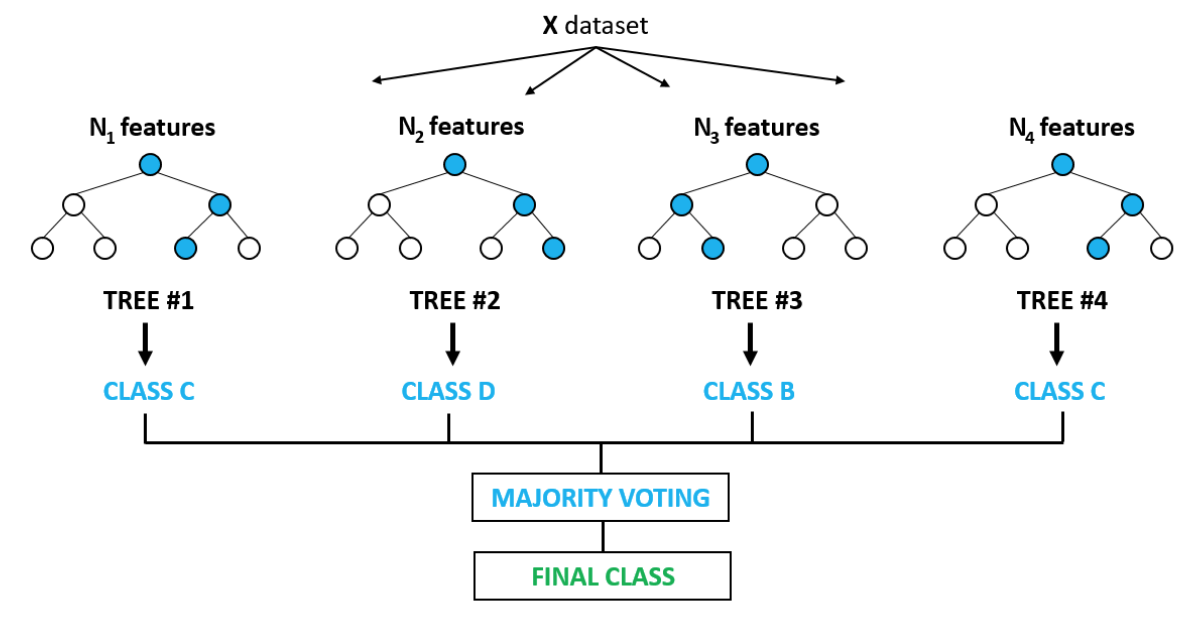
\includegraphics[width=9cm]{graphs/Random_Forest_description}
            \footnote{http://www.globalsoftwaresupport.com/random-forest-classifier-bagging-machine-learning/}
            \subsubsection{Support Vector Machine (SVM)}
            The Support Vector Machine (SVM) is a classifier that fits a line to the given data 
            similar to the way that a perceptron classifier does. The main difference between 
            these two is that the SVM algorithm specifies characteristics about the line that 
            cause it to fit the data better and allow for better generalized classifications that 
            the perceptron might not be able to achieve without significantly more data. The 
            algorithm specifies a line that separates the data in N-dimensional space, but line 
            must divide the data in such a way that the distance between the line and the next 
            adjoining datapoints, known as the margin, is maximized. The lines that run parallel 
            to the dividing line and run through the next adjoining data points are called the 
            support vectors, which is where the algorithm gets its name. For multi-class 
            classification the algorithm trains several lines to separate the different classes, 
            and then uses these lines to determine what class new data belongs to.
            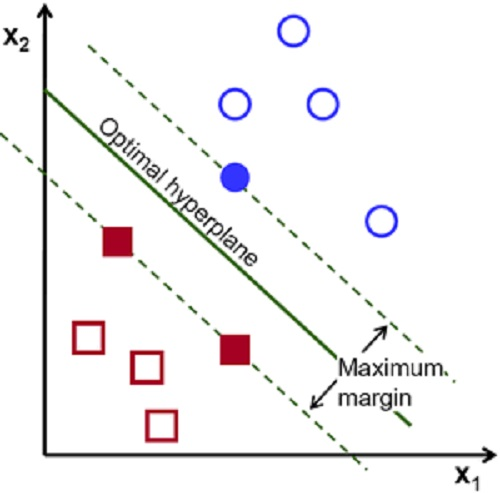
\includegraphics[width=7cm]{graphs/SVM_description}
            \footnote{https://aitrends.com/ai-insider/support-vector-machines-svm-ai-self-driving-cars/}
        
    \section{Initial Results}
        \subsection{Na\"ive Bayes}
        The initial results of Naïve Bayes were very promising. Naïve Bayes was run with two 
        different distributions. These distributions are a Multinomial distribution and a 
        Bernoulli Distribution. Below is a table with the results.
        \begin{center}
            \begin{tabular}{|cc|}
                \hline
                Multinomial & Bernoulli\\
                \hline
                0.9119      & 0.7451\\
                \hline
            \end{tabular}
        \end{center}
        The Multinomial Distribution ended up having the best overall accuracy. This is 
        because the Bernoulli distribution works better with discrete and boolean data rather 
        than the inverse document frequency counts that were used for training.
        \subsection{Random Forest}
        In order to get a better idea of the quality of the Random Forest classifier on the 
        news dataset, the algorithm was run with the default parameters. The most important 
        parameters are: criterion (gini or entropy), number of estimators (number of 
        different random trees that will vote), and min\_sample\_split (the minimum number of 
        samples required to split an internal node). The defaults were gini, 10 estimators, 
        and two samples required for splitting, resulting in an average accuracy of 0.8398 
        over five runs. 
        \subsection{Support Vector Machine (SVM)}
        The SVM algorithm, similar to Perceptron, has different functions that can be used to 
        model the dividing line in the data. Each is shown below along with the results of the 
        classification with that function:
        \begin{center}
            \begin{tabular}{|cc|}
                \hline
                Model   & Accuracy\\
                RBF     & 0.1352\\
                Poly    & 0.1212\\
                Sigmoid & 0.1077\\
                Linear  & 0.9373\\
                \hline
            \end{tabular}
        \end{center}
        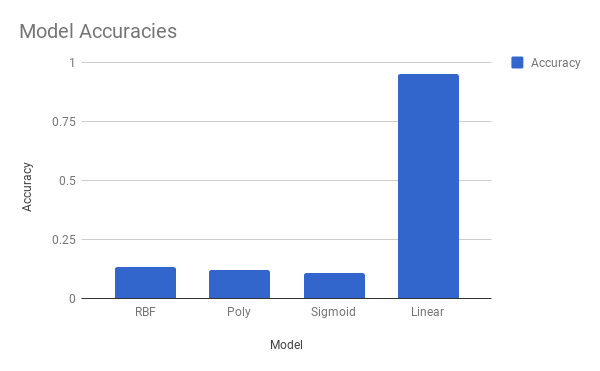
\includegraphics[width=9cm]{graphs/SVM_comparison}
        The linear model vastly outperformed the others. This is most likely because different 
        articles had word frequency values that strongly correlated with their subject, and so 
        the word vectors plotted in vector were linearly separable. The other models had 
        similar, poor, performance, which is likely because they tend to be used for 
        non-linear data, and using them for linearly separable data most likely lead to 
        significant overfitting.
        \subsection{Overall}
        From this initial analysis, SVM with the linear model seemed to yield the best results 
        of any of them. This is because SVM’s tend to work well in high-dimensional space. 
        Typically this is because we can use a ‘kernel trick’ in the SVM algorithm to 
        transform the data to look for higher order features that may be linearly separable. 
        However, in this case, that was unnecessary. Evidently, there were word frequency 
        values that correlated strongly enough with each document classification that new data 
        was largely linearly separable when plotted in N-dimensional space. This makes 
        intuitive sense, since seeing the word ‘Trump’, for example, would be strongly 
        correlated with the politics or satire classifications, and plotting these documents 
        in vector space would reflect that. Since Naïve Bayes uses probabilities to find its 
        results, and Random Forest splits on individual words, they may have produced similar 
        results by simply increasing the amount of data that we used.
        
    \section{Model Improvement}
    After seeing such high accuracies with the initial results, the parameters were adjusted to 
    see if the accuracy of the models could be improved.
        \subsection{Na\"ive Bayes}
        For Na\"ive Bayes, changing parameters were tested on both the Multinomial distribution 
        and the Bernoulli distribution. For both of the distributions, the parameter changed was 
        an alpha level. This alpha level corresponded to the smoothing rate that the distribution 
        would apply to the data. By changing this smoothing rate, it tries to connect missing data 
        points (places in the data where a number has not yet appeared) by making the fit more or 
        less tight.
        \begin{center}
            \begin{tabular}{|c|c|c|}
                \hline
                Smoothing Rate & Multinomial & Bernoulli \\
                \hline
                0.5 & 0.8911917098 & 0.7512953368 \\
                0.2 & 0.9150259067 & 0.7751295337 \\
                0.1 & 0.9279792746 & 0.8005181347 \\
                0.05 & 0.9119170984 & 0.810880829 \\
                0.01 & 0.8911917098 & 0.8077720207 \\
                0.001 & 0.8865284974 & 0.8046632124 \\
                \hline
            \end{tabular}
        \end{center}
        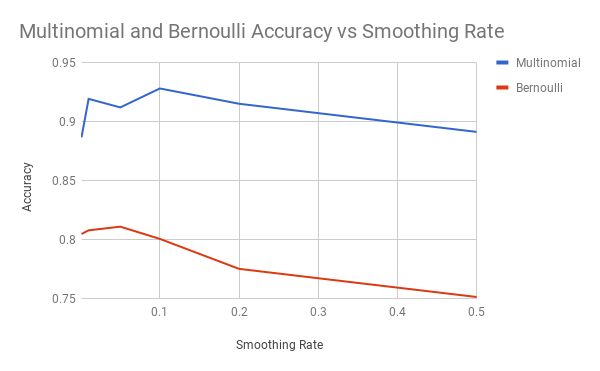
\includegraphics[width=9cm]{graphs/Naive_Bayes_comparison}
        In the graph, we can see that when the smoothing rate is too high or too low, the accuracy decreased. When the smoothing rate is too low, the probability distribution tries to overfit the training data that it has seen. When the smoothing rate is too high, the probability distribution loses some information about the probabilities and tries to treat values too similar to other numbers. As the graph also shows, the multinomial and bernoulli distributions were affected the same by the smoothing rate. This was expected since only the data was trying to be smoothed out and the distribution itself was still modeling the values given to it. In other words, both distributions reacted the same because missing data was trying to be filled in.
        \subsection{Random Forest}
        Using Scikit-Learn’s Random Search algorithm, we were able to train the model using 
        several combinations of values for the parameters mentioned above in order to improve the 
        accuracy. The table below shows the resulting accuracy of running the Random Forest tree 
        on different parameters. Note that the Sample Split column in the following table is the 
        Minimum size a sample needs to be to split.
        \begin{center}
            \begin{tabular}{|c|c|c|c|}
                \hline
                Sample Split & Criterion & Estimators & Mean Acc. \\
                \hline
                2 & gini & 10 & 0.8399 \\
                2 & gini & 275 & 0.9259 \\
                2 & entropy & 275 & 0.9067 \\
                10 & entropy & 50 & 0.8948 \\
                10 & entropy & 275 & 0.9114 \\
                10 & gini & 275 & 0.9233 \\
                \hline
            \end{tabular}
        \end{center}
        As shown above, keeping the default parameters the same, but increasing the number of 
        voters to 275 caused an improvement of almost 9\%. Note that 275 was used because it 
        produced the best results after running random search over several parameters. This 
        behavior was expected since the more models that are being trained, the higher the chances 
        of the majority correctly classifying the novel instance. With a higher number of 
        estimators, tuning the other parameters produced minimal changes. Using Gini Impurity as a 
        measure of the quality of splitting a node resulted in a better average accuracy than 
        regular entropy. The best results were found by using a minimum of 2 samples for 
        splitting, Gini Impurity, and 275 estimators, which resulted in 92.5\% of the test dataset 
        being correctly classified.
        \subsection{SVM}
        The main parameter used in SVM is a parameter called C. This parameter determines how much 
        the algorithm penalizes points being on the wrong side of the classification line. Thus, 
        high C would tend to lead to overfitting, while a low C would increase generalization and 
        ignore potential noise. The table below shows the results testing across different C 
        parameters:
        \begin{center}
            \begin{tabular}{|c|c|}
                \hline
                C       & Accuracy\\
                \hline
                0.1     & 0.7284\\
                1       & 0.9373\\
                10      & 0.9497\\
                100     & 0.945\\
                1000    & 0.9466\\
                \hline
            \end{tabular}
        \end{center}
        We had the best results at a C of 10, and it is interesting to note that increasing C by 
        orders of magnitude did little to change the results. Like we hypothesized earlier, this 
        data was most likely linearly separable and therefore did not have many points which were 
        on the wrong side of the classification line. This would mean that we would most likely 
        only see a significant drop in accuracy at very high levels of C. On the other hand, we 
        see a significant drop between a C of 1 and a C of .1. This is likely due to the program 
        trying to generalize too much and allowing for too many exceptions.\\
        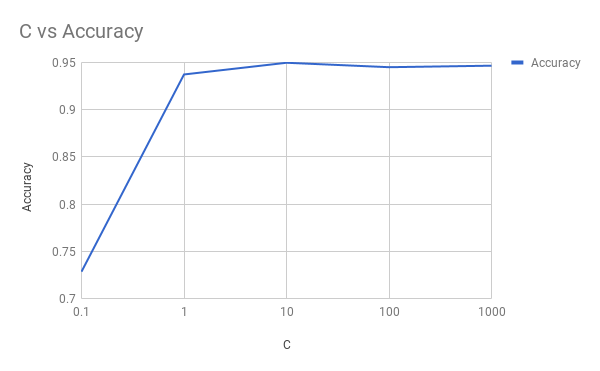
\includegraphics[width=9cm]{graphs/C_versus_accuracy}
        \indent{A second parameter that we tested was the shape of the decision functions, which 
        determines how many lines the SVM algorithm uses to separate the data. The two values for 
        this parameter are One vs One (OvO) and One vs Rest (OvR). One vs One trains a separate 
        classifier for each class individually against other individual classes, creating a total 
        of $\frac{N(N-1)}{2}$ classifiers, one for each class pair. One vs Rest, on the other 
        hand, trains a classifier for each class against all of the other classes collectively. 
        The results for this parameter are below:}
        \begin{center}
            \begin{tabular}{|c|c|c|}
                \hline
                            & OvO       & OvR\\
                \hline
                Accuracy    & 0.9450    & 0.9497\\
                \hline
            \end{tabular}
        \end{center}
        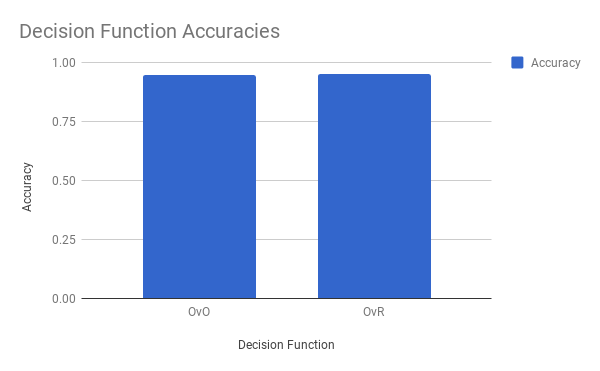
\includegraphics[width=9cm]{graphs/OvO_OvR}
        There is little difference between the results for these two parameters, but One vs Rest 
        did do better by a small margin. This could be due to simple chance since the accuracies 
        are so close, but it could also have to do with ambiguity between individual classes that 
        is not as apparent when considering all of the classes together. An example of this is 
        with the politics and satire classes. These may be difficult to tell apart, in some cases 
        even for humans, so a classifier meant to identify just the difference between these two 
        would have a hard time doing so. On the other hand, a classifier that had to distinguish 
        between politics and all the other classes collectively might have a greater chance of 
        success. Unsurprisingly, this classifier would still have trouble telling apart categories 
        such as politics or satire, which is why the differences between OvO and OvR are very 
        slight.
    
    \section{Final Results}
    Once again, SVM outperformed both of the other algorithms, but by less than before the 
    parameters were adjusted: Random Forest is the only algorithm that made a significant 
    improvement, reaching 0.9259 in its best case (as compared to its initial value of 0.8398). 
    However, SVM did make some progress (from an initial 0.9373 to 0.9497 at its best), and Na\"ive 
    Bayes also had a small improvement (from an initial 0.9119 to reaching 0.9259). These results 
    still show, though, that SVM was the best algorithm (as previously mentioned).

    \section{Future Work}
    Future work could include running a grid search to optimize the parameters used for each of 
    these things. By using grid search, we would be able to find the optimal parameters for each 
    algorithm and then be able to decide which algorithm was the best overall for our data 
    classification. We would also like to expand our dataset to include satirical articles of each 
    original classification to see if the algorithms could successfully determine between "fake" 
    news and actual articles.
\end{document}